\documentclass[../main/main.tex]{subfiles}

\newdate{date}{18}{12}{2019}


\begin{document}

\chapter{Widom's scaling theory. Block-spin Kadanoff's transformation}

\marginpar{ \textbf{Lecture 19.} \\  \displaydate{date}. \\ Compiled:  \today.}

\section{Introduction}
We have seen  that as a given system approaches a critical point \( T \rightarrow T_c^{\pm} \), the distance \( \xi  \)  over which the fluctuations of the order parameter are correlated becomes comparable to the size of the whole system \( L \) and the microscopic aspects of the system become irrelevant. This means that near a critical point the system has no longer characteristic lengths (\( a,L \)), besides \( \xi  \) of course that becomes the only relevant length scale of the problem. We can therefore expect that if we "move" a little bit from a critical point (\( t \sim 0 \)), for example changing the temperature by a small amount, the free energy of the system as a function will not change its shape, hence it is invariant in form by a change of scale.

 This hypothesis is also suggested by experimental data such as the ones shown by Guggenheim for the gas phase diagrams and the ones shown for ferromagnetic materials at different temperatures. Let us consider the experiment in Figure \ref{fig:19_2} (\cite{3_lesson_3} pag. 119); we can see that data from different temperatures, if scaled properly, collapse into two (one for \( t<0 \) and one for \( t>0 \)) unique curves. It is clearly illustrated in Figure \ref{fig:19_1}. At the origin, the Widom's static scaling theory was introduced also to explain this collapse.

 \begin{figure}[h!]
 \centering
 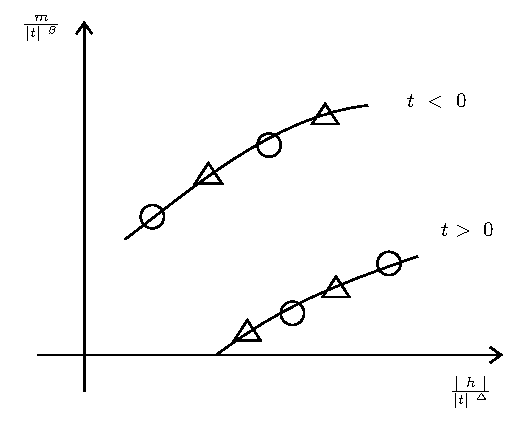
\includegraphics[width=0.55\textwidth]{../lessons/19_image/1.pdf}
 \caption{\label{fig:19_1} Scaled magnetization \( m \) is plotted against scaled magnetic field \( h \).}
 \end{figure}

 \begin{figure}[h!]
 \centering
 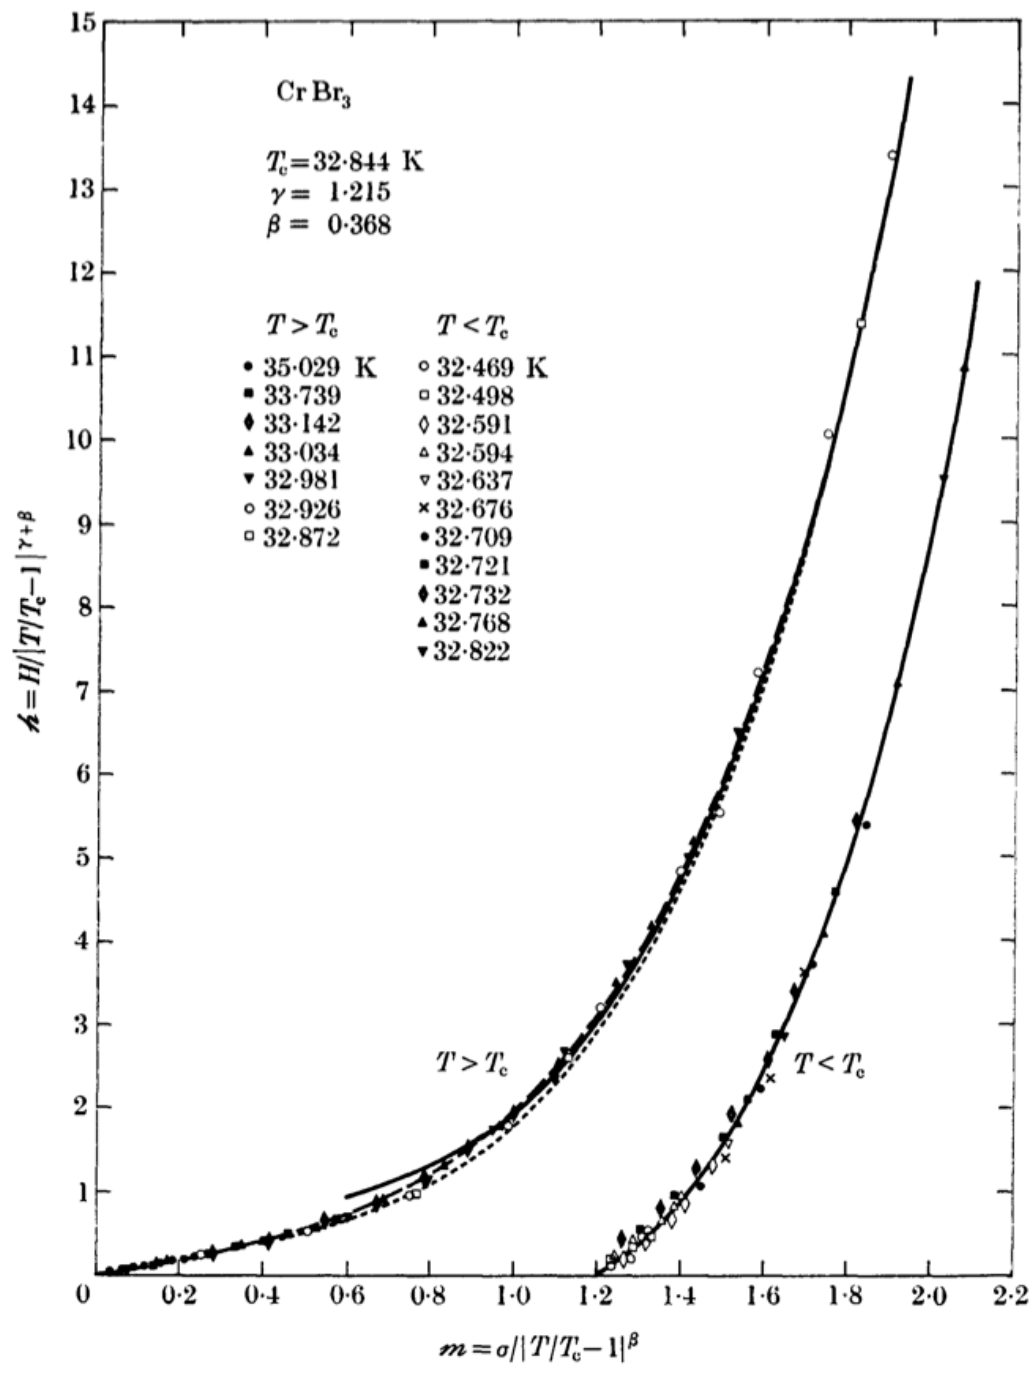
\includegraphics[width=0.7\textwidth]{../lessons/19_image/exp.jpg}
 \caption{\label{fig:19_2} Scaled magnetic field \( h \) is plotted against scaled magnetization \( m \) for the insulating ferromagnet \( \text{CrBr}_3 \), using data from seven supercritical \( (T>T_c) \) and from eleven subcritical \( T<T_c \) isotherms. Here \( \sigma \equiv M/M_0 \). (1969) \cite{3_lesson_3}}
 \end{figure}




\section{Widom's static scaling theory}
We have seen that when a phase transition occurs the free energy of the system is such that the response functions exhibit singularities, often in the form of divergences. To make a concrete example (but of course all our statements are completely general) if we consider a magnetic system we can suppose to write its free energy density as:
\begin{equation*}
  f(T,H) = f_r (T,H) + f_s (T,H)
\end{equation*}
where \( t = (T-T_c)/T_c \) and \( h = (H-H_c)/k_B T \), \( f_r \)  is the "regular" part of the free energy (which does not significantly change near a critical point, it is an analytic function), while \( f_s \) is the "singular" one, which contains the non-analytic behaviour of the system near a critical point (i.e. \( t \sim 0 \) and \( h \sim 0 \)).

Widom's static scaling hypothesis consists in assuming that the singular part \( f_s \) of the free energy is a generalized homogeneous function, i.e.:
\begin{equation*}
  f_s (\lambda ^{p_1}t, \lambda ^{p_2} h) = \lambda f _s (t,h), \quad \forall \lambda \in \R
\end{equation*}
Note that assuming that one thermodynamic potential is a generalized homogeneous function implies that all the other thermodynamic potentials are so.

Therefore, in order to properly define the scaling hypothesis, we should rely on the mathematical concept of homogeneous functions and now we discuss the main properties of such functions.



\subsection{Homogeneous functions of one or more variables}

\subsubsection{Single variable}
Let us begin with the definition of homogeneous function for a single variable \( r \).
\begin{definition}{Homogeneous function}{}
A function \( f(r) \) is said to be homogeneous in \( r \) if
\begin{equation}
  f (\lambda r) = g (\lambda ) f(r), \qquad \forall \lambda \in \R
\end{equation}
where \( g \) is, for the moment, an unspecified function (we will shortly see that it has a precise form).
\end{definition}
\begin{example}{Parabola \( \pmb{ f(r) = B r^2} \) }{}
  An example of homogeneous function is
\begin{equation*}
  f(r) = B r^2
\end{equation*}
in fact
\begin{equation*}
  f ( \lambda r) = B ( \lambda r)^2 = \lambda ^2 f (r)
\end{equation*}
and so in this case \( g ( \lambda ) = \lambda ^2 \).
\end{example}

A very interesting property of an homogeneous functions is that,  once its value in a point \( r_0 \) (i.e. \( f(r_0) \)) and the function \( g(\lambda ) \) are known,
the entire \( f(r) \) can be reconstructed for all \( r \in \R \); indeed, any \( r \) can be written in the form \( r=\lambda r_0 \) (of course with \( \lambda = r / r_0 \)), so that
\begin{equation}
  f(r) = f (\lambda r_0) = g(\lambda ) f(r_0)
\end{equation}
We now want to show that \( g (\lambda ) \)  has a precise form.


\begin{theorem}{}{}
  The function \( g(\lambda ) \) is not arbitrary, but it must be of the form
\begin{equation}
  g(\lambda ) = \lambda ^p
\end{equation}
where \( p \) is the degree of the homogeneity of the function.
\end{theorem}

\begin{proof}
  From the definition of homogeneous function, for \( \lambda, \mu \in \R  \) we have on one hand that:
\begin{equation*}
  f(\lambda \mu r) = f(\lambda (\mu r)) = g (\lambda ) f(\mu r) = g(\lambda ) g(\mu ) f(r)
\end{equation*}
on the other hand,
\begin{equation*}
  f((\lambda \mu )r) = g (\lambda  \mu ) f(r)
\end{equation*}
and so:
\begin{equation*}
  g (\lambda \mu ) = g(\lambda ) g (\mu )
\end{equation*}
If we now suppose \( g \) to be differentiable\footnote{Actually \( g(\lambda ) \) continuous is sufficient, but proof becomes more complicated.}, then differentiating with respect to \( \mu  \)  this last equation we get:
\begin{equation*}
  \pdv{}{\mu } \qty[g(\lambda \mu )] = \pdv{}{\mu } \qty[ g(\lambda )g(\mu  )] \quad
  \Rightarrow \lambda g' (\lambda \mu ) = g (\lambda ) g' (\mu )
\end{equation*}
Setting \( \mu =1 \) and defining \( p \equiv g'( \mu =1 ) \), we have:
\begin{equation*}
   \lambda g'(\lambda ) = g(\lambda ) p \quad \Rightarrow \frac{g'(\lambda )}{g(\lambda )} = \frac{p}{\lambda }
\end{equation*}
which yields:
\begin{equation*}
  \dv{}{\lambda } \qty(\ln{g(\lambda )} ) = \frac{p}{\lambda }   \quad \Rightarrow \ln{g(\lambda )} = p \ln{\lambda } + c \quad \Rightarrow g (\lambda ) = e^c \lambda ^p
\end{equation*}
Now, \( g'(\lambda ) = p e^c \lambda ^{p-1} \), so since \( g'(1) = p \) by definition we have  \( p = p e^c \) and thus \( c=0 \).
Therefore:
\begin{equation*}
  g(\lambda ) = \lambda ^ p
\end{equation*}
A homogeneous function such that \(   g(\lambda ) = \lambda ^ p \)  is said to be homogeneous of degree \( p \).
\end{proof}

\subsubsection{Generalized homogeneous functions (more variables)}
Let us now define homogeneous functions for more than only one variable:
\begin{equation*}
  f(\lambda x, \lambda y) = \lambda ^p f(x,y), \quad \forall \lambda \in \R
\end{equation*}
 The function  \( f(x,y) \) is a \emph{generalized homogeneous function} if has as more general form
\begin{empheq}[box=\myyellowbox]{equation}
  f (\lambda ^a x, \lambda ^b y) = \lambda f(x,y), \quad \forall \lambda \in \R
  \label{eq:19_2}
\end{empheq}


\begin{remark}
  If we consider instead
  \begin{equation*}
      f (\lambda ^a x, \lambda ^b y) = \lambda^p f(x,y)
  \end{equation*}
  we can always choose \( \lambda ^p \equiv s \) such that
  \begin{equation*}
    f ( s^{a/p} x, s^{b/p} y) = s f(x,y)
  \end{equation*}
  and choosing \( a'=a/p \) and \( b'=b/p \) we are back to \eqref{eq:19_2}. Hence, it is the most general form an homogeneous function can have.
\end{remark}


\begin{remark}
Since \( \lambda  \) is arbitrary, we can choose \( \lambda  = y ^{-1/b} \), thus we get
\begin{equation*}
  f(x,y) = y^{1/b} f \qty( \frac{x}{y^{a/b}},1)
\end{equation*}
in that way \( f \) depends on \( x \) and \( y \) only through the ratio \( \frac{x}{y^{a/b}} \)! Similarly, for \( x \), one can choose \( \lambda = x^{-1/a} \), obtaining
\begin{equation*}
  f(x,y) = x^{1/a} f \qty(1, \frac{y}{x^{b/a}})
\end{equation*}

\end{remark}
\begin{example}{}{}
The function \( f(x,y) = x^3 + y^7 \) is an homogeneous one. Indeed, we have:
\begin{equation*}
  f(\lambda ^{1/3} x, \lambda ^{1/7}y) = \lambda x^3 + \lambda y^7 = \lambda f (x,y)
\end{equation*}
Instead, examples of non-homogeneous functions are:
\begin{equation*}
  f(x) = e^{-x}, \qquad f(x) = \log{x}
\end{equation*}

\end{example}





\subsection{Widom's scaling hypothesis}

As said, the Widom's static scaling hypothesis consists in assuming that the singular part of the free energy, \( f_s \), is a generalized homogeneous function, i.e.:
\begin{empheq}[box=\myyellowbox]{equation}
  f_s ( \lambda ^{p_1} t, \lambda ^{p_2} h) = \lambda f_s (t,h), \quad \forall \lambda \in \R
\end{empheq}
where \( p_1 \) and \( p_2 \) are the degrees of the homogeneity.

The exponents \( p_1 \)  and \( p_2 \) are not specified by the scaling hypothesis; however, we are shortly going to show that all the critical exponents of a system can be expressed in terms of \( p_1 \)  and \( p_2 \); this also implies that if two critical exponents are known, we can write \( p_1 \) and \( p_2 \) in terms of them (since in general we will have a set of two independent equations in the two variables \( p_1 \) and \( p_2 \)  and therefore determine all the critical exponents of the system. In other words, we just need to know two critical exponents to obtain all the others.

\begin{remark}
Since \( f_s \) is a generalized homogeneous function, it is always possible to choose \( \lambda  \) to remove the dependence on one of their arguments;
for example, one can choose \(   \lambda = h^{-1/p_2} \) to obtain
\begin{equation*}
 f_s (t,h) = h^{1/p_2} f_s (h^{-p_1/p_2} t , 1)
\end{equation*}
where
\begin{equation*}
  \Delta  \equiv \frac{p_2}{p_1}
\end{equation*}
is called the \emph{gap exponent}.
\end{remark}



\section{Relations between critical exponents}
Let us now explore the consequences of Widom's assumption on the critical exponents of a system, again on a magnetic one for concreteness. Indeed, let us see how this simple hypothesis allow us, by simple differential calculus, to obtain relations between the thermodynamic critical exponents.

\subsection{Exponent \( \pmb{\beta } \) (scaling of the magnetization)}
Let us start from the scaling hypothesis
\begin{equation*}
  f_s (\lambda ^{p_1}t, \lambda ^{p_2}h) = \lambda f_s (t,h)
\end{equation*}
Since
\begin{equation*}
  M = \pdv{f}{H}
\end{equation*}
deriving both sides of Widom's assumption with respect to \( h \)\footnote{We should in principle derive with respect to \( H \), but since \( h \propto \beta H \), the  \( \beta  \) factors simplify on both sides.} we get:
\begin{equation*}
  \lambda ^{p_2} \pdv{f_s}{h} \qty(\lambda ^{p_1}t, \lambda ^{p_2}h) = \lambda \pdv{f_s}{h} (t,h)
\end{equation*}
and thus:
\begin{equation*}
   \lambda ^{p_2} M_s ( \lambda ^{p_1} t, \lambda ^{p_2} h) = \lambda M_s (t,h)
\end{equation*}
On the other hand, we know that, for \( h=0 \) and \( t \rightarrow 0^- \), \( M_s (t) \sim (-t)^{\beta } \). Hence, in order to determine \( \beta  \), we set \( h=0 \) so that this becomes
\begin{equation*}
  M_s (t,0) = \lambda ^{p_2 -1} M_s ( \lambda ^{p_1} t,0)
\end{equation*}
Since \( \lambda  \) is arbitrary, using the properties of generalized homogeneous functions, we set
\begin{equation*}
  \lambda ^{p_1} t = -1 \quad \Rightarrow \lambda = (-t)^{-1/p_1}
\end{equation*}
to eliminate the dependence on \( t \). Hence, we get
\begin{equation*}
  M_s (t,0) =  (-t)^{(1-p_2)/p_1} M_s (-1,0)
\end{equation*}
By definition of the \( \beta  \) critical exponent, we have:
\begin{equation}
  \beta = \frac{1-p_2}{p_1}
  \label{eq:19_10}
\end{equation}


\subsection{Exponent \( \pmb{\delta}  \)}
Let us consider again the relation
\begin{equation*}
   \lambda ^{p_2} M_s ( \lambda ^{p_1} t, \lambda ^{p_2} h) = \lambda M_s (t,h)
\end{equation*}
We can determine the exponent \( \delta  \) by setting \( t=0 \) (\( T=T_c  \)), obtaining:
\begin{equation*}
  M(0,h) = \lambda ^{p_2-1} M (0, \lambda ^{p_2} h)
\end{equation*}
Now, using again the same property of generalized homogeneous functions we set
\begin{equation*}
  \lambda ^{p_2} h = 1 \quad \Rightarrow \lambda = h^{-1/p_2}
\end{equation*}
and we get:
\begin{equation*}
  M_s (0,h) =  h^{(1-p_2)/p_2} M_s (0,1)
\end{equation*}
Since \(  M_s  \overset{h \rightarrow 0^+}{\sim} h^{1/\delta } \), we have:
\begin{equation}
  \delta = \frac{p_2}{ 1 - p_2 }
  \label{eq:19_11}
\end{equation}

Now we can also express \( p_1 \) and \( p_2 \)  in terms of \( \beta  \) and \( \delta  \) from the two relations Eq.\eqref{eq:19_10} and Eq.\eqref{eq:19_11}. The result is:
\begin{equation}
  p_1 = \frac{1}{\beta (\delta +1)}, \qquad p_2 = \frac{\delta }{\delta + 1}
\end{equation}
from which we see that the gap exponent is:
\begin{equation}
  \Delta \equiv \frac{p_2}{p_1}  = \beta \delta
\end{equation}


\subsection{Exponent \( \pmb{\gamma  } \) }
In order to obtain the magnetic susceptibility, we derive twice the expression of Widom's assumption with respect to \( h \), to get:
\begin{equation*}
  \lambda ^{2p_2} \chi _T \qty(\lambda ^{p_1}t, \lambda ^{p_2}h) = \lambda \chi _T (t,h)
\end{equation*}

The exponent \( \gamma   \) describes the behaviour of \( \chi _T \)  for \( t \rightarrow 0 \)  when no external field is present (\( h=0 \)). What we can now see is that the scaling hypothesis leads to the equality of the exponents for \( t \rightarrow 0^+ \)  and \( t \rightarrow 0^- \).

\begin{itemize}
\item Case \( t \rightarrow 0^- \): setting \( h=0 \)  and \( \lambda = (-t)^{-1/p_1} \) we get
\begin{equation*}
  \chi _T (t,0) = \qty(-t)^{-\frac{2p_2-1}{p_1}} \chi _T (-1,0)
\end{equation*}
and if we call \( \gamma ^-  \)  the critical exponent for \( t \rightarrow 0^- \), we see that, since
\begin{equation*}
  \chi _T (t,0) \overset{t \rightarrow 0^-}{\sim } \qty(-t)^{-\gamma_-  }
\end{equation*}
we get
\begin{equation*}
  \gamma _- = \frac{2p_2 -1}{p_1} = \beta (\delta -1)
\end{equation*}

\item Case \( t \rightarrow 0^+ \): setting \( h=0 \)  and \( \lambda = (t)^{-1/p_1} \) we get
\begin{equation*}
  \chi _T (t,0) = t^{-\frac{2p_2-1}{p_1}} \chi _T (1,0)
\end{equation*}
and if we call \( \gamma ^+  \)  the critical exponent for \( t \rightarrow 0^+ \), we see that, since
\begin{equation*}
  \chi _T (t,0) \overset{t \rightarrow 0^+}{\sim } t^{-\gamma_+  }
\end{equation*}
we get
\begin{equation*}
  \gamma _+ = \frac{2p_2 -1}{p_1} = \beta (\delta -1)
\end{equation*}
\end{itemize}
We therefore see explicitly that:
\begin{equation}
  \gamma _- = \gamma _+ \equiv \gamma  = \frac{2p_2 -1}{p_1} = \beta (\delta -1)
\end{equation}





\subsection{Exponent \( \pmb{\alpha } \) (scaling of the specific heat)}
In order to determine the behaviour of the specific heat (at constant external field) near the critical point, we derive the expression of Widom's assumption twice with respect to the temperature \( t \), so that:
\begin{equation*}
  \lambda ^{2p_1}c_H \qty(\lambda ^{p_1}t, \lambda ^{p_2}h) = \lambda c_H (t,h)
\end{equation*}
We want to see again that the scaling hypothesis leads to the equality of the exponents for \( t \rightarrow 0^+ \)  and \( t \rightarrow 0^- \).

\begin{itemize}
\item Case \( t \rightarrow 0^- \): setting \( h=0 \) and \( \lambda = (-t)^{-1/p_1} \) we get
\begin{equation*}
  c_H (t,0) = \qty(-t)^{-\qty(2- \frac{1}{p_1}) } c_H (-1,0)
\end{equation*}
and if we call \( \alpha ^-  \)  the critical exponent for \( t \rightarrow 0^- \), we see that, since
\begin{equation*}
  c_H (t,0) \overset{t \rightarrow 0^-}{\sim } (-t)^{-\alpha _-}
\end{equation*}
we get
\begin{equation*}
  \alpha _- = 2 - \frac{1}{p_1}
\end{equation*}

\item Case \( t \rightarrow 0^+ \): setting \( h=0 \) and \( \lambda = (t)^{-1/p_1} \) we get
\begin{equation*}
  c_H (t,0) = t^{-\qty(2- \frac{1}{p_1}) } c_H (1,0)
\end{equation*}
and if we call \( \alpha ^+  \)  the critical exponent for \( t \rightarrow 0^+ \), we see that, since
\begin{equation*}
  c_H (t,0) \overset{t \rightarrow 0^-}{\sim } t^{-\alpha _+}
\end{equation*}
we get
\begin{equation*}
  \alpha _+ = 2 - \frac{1}{p_1}
\end{equation*}

\end{itemize}

We have again:
\begin{equation}
  \alpha  _- = \alpha  _+ \equiv \alpha  = 2 - \frac{1}{p_1}
  \label{eq:19_6}
\end{equation}




\subsection{Griffiths and Rushbrooke's equalities}
\label{sec:19_1}
If we now substitute \( p_1 = \frac{1}{\beta (\delta +1)} \) into \( \alpha  =  2 - \frac{1}{p_1} \), we get:
\begin{empheq}[box=\myyellowbox]{equation}
  \alpha + \beta (\delta +1) = 2
\end{empheq}
This is the \emph{Griffiths equality}, which we have already encountered in inequalities between critical exponents as an inequality (see Sec.\ref{sec:3_2}).

On the other hand, \emph{Rushbrooke's equality} is obtained by combining Griffith equality with the relation \( \gamma = \beta (\delta -1)  \):
\begin{empheq}[box=\myyellowbox]{equation}
\alpha + 2 \beta + \gamma = 2
\end{empheq}
We therefore see, as anticipated in Sec.\ref{sec:3_2}, that the static scaling hypothesis allows to show that they are indeed exact equalities.




\subsection{An alternative expression for the scaling hypothesis}
We can re-express Widom's assumption in another fashion often used in literature. Let us consider the Widom's assumption
\begin{equation*}
  f_s ( \lambda^{p_1} t, \lambda ^{p_2}h) = \lambda f_s (t,h)
\end{equation*}
If we set \( \lambda = t ^{-1/p_1} \), then:
\begin{equation*}
  f_s (1,t^{-p_2/p_1}h) = t^{-1/p_1} f_s (t,h)
\end{equation*}
From \( \Delta = \frac{p_2}{p_1} \) and \( \alpha = 2 - \frac{1}{p_1} \), we can rewrite this as:
\begin{equation}
  f_s (t,h) = t^{2- \alpha } f_s \qty(1, \frac{h}{t^{\Delta }})
\end{equation}
which is the most used form of the scaling hypothesis in statistical mechanics.

As we can notice, we have not considered the critical exponents \( \eta  \)  and \( \nu  \); this will be done shortly in Kadanoff's scaling and correlation lengths.

\subsection{Scaling of the equation of state}
Besides the relations between critical exponents, Widom's static scaling theory allows us to make predictions on the shape of the state equation of a given system.
By predicting the scaling form of the equation of state, we can explain the collapse of the experimental data. Let us now see how, again for a magnetic system. We start from the relation
\begin{equation*}
  M_s (t,h) = \lambda ^{p_2 - 1} M_s (\lambda ^{p_1} t, \lambda ^{p_2} h)
\end{equation*}
Using the property of generalized homogeneous functions we set \( \lambda = \abs{t}^{-1/p_1}  \). Hence,
\begin{equation*}
  M_s (t,h) = \abs{t}^{\frac{1-p_2}{p_1}} M_s ( \frac{t}{\abs{t} }, \frac{h}{\abs{t}^{p_2/p_1 } })
\end{equation*}
Since \( \beta = (1-p_2)/p_1 \) and \( \Delta = p_2/p_1 \), we have
\begin{equation}
  \frac{M_s (t,h)}{\abs{t}^{\beta } } = M_s ( \frac{t}{\abs{t} }, \frac{h}{\abs{t}^{\Delta } })
  \label{eq:19_5}
\end{equation}
Hence, we can define the \emph{scaled magnetization} and \emph{scaled magnetic field}  as
\begin{equation}
    \bar{m} \equiv \abs{t}^{-\beta } M(t,h), \qquad \bar{h} \equiv \abs{t}^{-\Delta } h (t,M)
\end{equation}
and
\begin{equation}
  F_{\pm} ( \bar{h} ) \equiv M_s (\pm1, \bar{h} )
\end{equation}
where \( +1 \)  corresponds to \( t>0 \)  (namely \( T>T_c \)) and \( -1 \)  to \( t<0 \)  (i.e. \( T<T_c \)).
Using these definitions, Eq.\eqref{eq:19_5} becomes
\begin{equation}
  \bar{m} = F_{\pm} (\bar{h} )
\end{equation}
The meaning of this equation is that if we measure \( M \) and \( h \) and rescale them as we have just seen, all the experimental data should fall on the same curve independently of the temperature \( T \); there are of course two possible curves (not necessarily equal), one for \( T>T_c \)  and one for \( T<T_c \)  (which correspond to \( M(1,h) \) and \( M(-1,h) \)). These predictions are in perfect agreement with experimental results shown in Figure \ref{fig:19_2}, and are one of the greatest successes of Widom's static scaling theory.






\section{Kadanoff's block spin and scaling of the correlation function}
As we have seen, Widom's static scaling theory allows us to determine exact relations between critical exponents, and to interpret the scaling properties of systems near a critical point. However, this theory is based upon the following equation:
\begin{equation*}
  f (T,H) = f_r (T,H) + f_s(T,H)
\end{equation*}
but gives no physical interpretation of it; in other words, it does not tell anything about the physical origin of scaling laws. Furthermore, as we have noticed Widom's theory does not involve correlation lengths, so it tells nothing about the critical exponents \( \nu  \)  and \( \eta  \).



We know (see Long range correlations) that one of the characteristic traits of critical phenomena is the divergence of the correlation length \( \xi  \), which becomes the only physically relevant length near a critical point. However, by now we are unable to tell if and how this is related to Widom's scaling hypothesis; everything will become more clear within the framework of The Renormalization Group, in which we will see that Widom's assumption is a consequence of the divergence of correlation length.

Widom's theory refers only to the free energy of the system. Moreover it do, not fully explain how the scaling hypothesis derives by \( \xi  \) being the only relevant length of the system.

The first argument on this point was given \( 1966 \) by Kadonoff.
The Kadonoff's intuition was: the divergence of \( \xi  \) implies a relation between the coupling constants of a \( \mathcal{H}_{eff} \) and the length scales over which \( m \) is defined.

We will that Kadanoff's intuition is correct. However, the relation found by Kadanoff is an approximation of the one proposed later by the theory of renormalization.
\begin{remark}
How can we relate the coupling costant of the two hamiltonian. This is the idea of the renormalization group. (lesson)
\end{remark}
\subsection{Kadanoff's argument}
It is based on a coarse-grained operation on the system and two basic assumptions.
\subsubsection{Coarse graining operation}
Let us start from the Hamiltonian
\begin{equation}
  - \beta \mathcal{H}_{\Omega } = k \sum_{\expval{ij} }^{} \sigma _i \sigma _j + h \sum_{i}^{} \sigma _i
\end{equation}
with
\begin{equation}
  \sigma _i = \pm 1, \quad k \equiv \frac{J}{k_B T}, \quad h \equiv \frac{H}{k_B T}
\end{equation}
Given \( xi \) we know that, for distances \( r < \xi  \), the spins are correlated.

Let partition the system into blocks of size \( la \) (\( a \) is the lattice unit length while \( l \) is a adimensional scale) such that
\begin{equation}
  r \ll \xi  \quad \Rightarrow a \ll l a \ll \xi (t)
\end{equation}
The coarse-graining procedure consits in substituting the spins \( \sigma _i \) in a block of length \( la \) with a \emph{superspin} or \emph{block spin} \( S_I \).

The transformation chosen by Kadanoff was the following
\begin{equation}
  S_I \equiv \frac{1}{\abs{m_l} } \frac{1}{l^D} \sum_{i \in I}^{}  \sigma _i
  \label{eq:19_7}
\end{equation}
where \( m_l \) is the average magnetization of the \( I \)-esim block
\begin{equation}
  m_l \equiv \frac{1}{l^D} \sum_{i \in I}^{} \sigma _i
\end{equation}
with the sum that is over all the sites with a given cell.
\begin{remark}
The division by \( \abs{m_l}  \) in equation \eqref{eq:19_7} is crucial because it rescales the new variables \( S_I \) to have the original values \( \pm 1 \) (rescaling of the fields).
\end{remark}

\subsubsection{\(  1^{st} \) crucial assumption}
The frist assumption is that the Hamiltonian of the new system \( \mathcal{H}_l \) is equal in form to \( \mathcal{H}_ \Omega  \), the original one:
\begin{equation}
  - \beta \mathcal{H}_l = k_l \sum_{\expval{IJ} }^{N_b} S_I S_J  + h_l \sum_{I=1}^{N_b} S_I
\end{equation}
\begin{remark}
This assumption is in general wrong!
\end{remark}
Only the coupling constants \( k_l \) and \( h_l \) can change by the transformation. Note that the number of block spins \( N_l \) is given by \(   N_l = \frac{N}{l^D} \).

How you measure in the new system the lengths? the correlations lengths. Before we have changed the size of the system. We have increased the ruler, so the number is smaller now. It seems stupid but it is fundamental.
An important point is: the new system has a lattice length equal to \( la \), hence in the new system all the lengths will be measured in units of \( la \). In particular
\begin{equation}
  \xi _l = \frac{\xi }{l}
\end{equation}
that is \( \xi _l \) has a numerical value smaller than the one measured in the original lattice.

What does it mean? Since \( \xi _l < \xi  \) the system described by \( \mathcal{H}_l \)   is more distant from the critical point than the original \( \mathcal{H} (\sigma _i) \)! We should expect \( t_l > t \).

Similarly, \( h_l \) will be such that
\begin{equation}
  h \sum_{i}^{} \sigma _i = h \sum_{I}^{} \sum_{i \in \sigma _i}^{}  \sigma _i = h \sum_{I}^{}    \abs{m_l} l^D S_I
  = \underbrace{h \abs{m_l} l^D}_{h_l} \sum_{I}^{} S_I \equiv  h_l \sum_{I}^{} S_I
\end{equation}
giving
\begin{equation}
  h_l = \abs{m_l} l^D h
\end{equation}
Since \( \mathcal{H}_l \) is equal in form to \( \mathcal{H} \), so it is \( Z_l \) and hence the free energies per spins satisfy the equation
\begin{equation}
  N_l f_s (t_l,h_l) = N f_s (t,h)
\end{equation}
Hence,
\begin{equation}
  \Rightarrow  f_s (t_l,h_l) = l^D f_s (t,h)
\end{equation}
Note that the homogeneity condition is recovered with \( \lambda \equiv l^D \).
We now should ask how \( t \) and \( h \) change under the block spin transformation.

\subsubsection{\(  2^{st} \) crucial assumption}
The second assumption is
\begin{equation}
  \begin{cases}
     t_l = t l^{Y_t}\\
  h_l = h l^{Y_h}
  \end{cases}
  \label{eq:19_8}
\end{equation}
where \( Y_t, \, Y_h \) are scaling exponents and are unknown!
Inserting \eqref{eq:19_8} in the free energy equation one obtains
\begin{equation}
  f_s (t,h) = l^{-D} f_s (t l^{Y_t}, h l^{Y_h})
\end{equation}
As the parameter \( \lambda  \), in Widom also \( l \)  can be chosen such that
\begin{equation}
  l= \abs{t}^{-1/Y_t}
\end{equation}
so
\begin{equation}
  f_s (t,h) = \abs{t}^{D/Y_t} f_s (1, h \abs{t}^{-Y_h/Y_t} )
\end{equation}
Therefore,
\begin{equation}
  \Delta = \frac{Y_h}{Y_t}
\end{equation}
\begin{remark}
By comparing with the Widom's scaling
\begin{equation}
  f_s (t,h) \sim t^{2- \alpha } f_s \qty(1, \frac{h}{t^\Delta})
\end{equation}
we get the new relation
\begin{equation}
  2 - \alpha = \frac{D}{Y_t}
\end{equation}
\end{remark}


\section{Kadanoff's argument applied to the two-point correlation}
Let us compute the two-point correlation function for the block spins
\begin{equation}
  G_{IJ} (\va{r}_l, t_l) \equiv \expval{S_I S_J} - \expval{S_I}\expval{S_J}
\end{equation}
Since
\begin{equation}
  h_l = h \abs{m_l} l^D \quad \Rightarrow \abs{m_l} = \frac{h_l l^{-D}}{h}
\end{equation}
and using \( h_l = h l^{Y_h} \), we obtain
\begin{equation}
  \abs{m_l} = l^{\frac{1}{h}-D}
\end{equation}
Since
\begin{equation}
  S_I = \frac{1}{\abs{m_l} } \frac{1}{l^D} \sum_{i \in I}^{} \sigma _i
\end{equation}
we have
\begin{equation}
\begin{split}
  G_{IJ} (\va{r}_l, t_l) &=  \expval{S_I S_J} - \expval{S_I} \expval{S_J}    \\
  & = \frac{1}{l^{2 (Y_h - D)} l^{2D}} \sum_{i \in I}^{} \sum_{j \in J}^{} \qty[ \underbrace{\expval{\sigma _i \sigma _j} - \expval{\sigma _i} \expval{\sigma _j} }_{ (a) }    ] \\
  & = \frac{l^D l^D}{l^{2(Y_h-D)}l^{2D}} \qty[ \expval{\sigma _i \sigma _j} - \expval{\sigma _i} \expval{\sigma _j}  ]
\end{split}
\end{equation}
in fact \( (a) \) we have made the assumption  that since \( la \ll \xi  \), \( G_{ij} \) inside a block is fairly constant
\begin{remark}
  \begin{equation}
    \abs{\va{r}_l} = \frac{\va{r}}{l}
  \end{equation}
\end{remark}
Hence,
\begin{equation}
  G_{IJ} (\va{r}_l, t_l) = l^{2(D-Y_h)} G_{ij} (\va{r},t)
\end{equation}
If one includes also the \( h \) dependence:
\begin{equation}
  G_{IJ} \qty(\frac{\va{r}}{l}, t l^{Y_t}, h l^{Y_h}) = l^{2 (D- Y_h)} G_{ij} (\va{r},t,h)
 \end{equation}
By choosing \(   l = t^{-1/Y_t} \) one gets
\begin{equation}
  G (\va{r},t,h) = t^{\frac{2(D-Y_h)}{Y_t}} G (\va{r}t^{1/Y_t}, 1 , h t ^{-Y_h/Y_t})
  \label{eq:19_9}
\end{equation}
Since we are interested at large length scale in proximiti of \( T=T_c \), we can choose \( \abs{\va{r}}  \) such that
\begin{equation}
  \abs{\va{r}} t^{1/Y_t} = 1  \quad \Rightarrow  t = \abs{\va{r}}^{-Y_t}
\end{equation}
Hence, inserting in \eqref{eq:19_9}
\begin{equation}
  G (\va{r},t,h) = \abs{\va{r}}^{-2(D-Y_h)} F_G \qty(h t^{-Y_h/Y_t})
\end{equation}
where
\begin{equation}
  F_G \qty(h t^{-Y_h/Y_t})  \equiv G (1, h t ^{-Y_h/Y_t},1)
\end{equation}

Remembering the power law behaviour of \( G \) in proximity of the critical point, i.e.  \( G \sim \abs{\va{r}}^{2-D- \eta }  \) and \( \xi \sim t^{-\nu } \).
Finally we get
\begin{equation}
  \nu = \frac{1}{Y_t}, \quad 2 (D- Y_h) = D - 2 + \eta
\end{equation}
Hence, we obtain the hyperscaling relation
\begin{equation}
      \Rightarrow 2 - \alpha = \nu D
\end{equation}





\end{document}
